% \documentclass[a4paper,12pt]{extarticle}

% % =========================
% % Page layout (Annex 7)
% % =========================
% \usepackage[
%   left=2.5cm,
%   right=1.0cm,
%   top=2.0cm,
%   bottom=2.0cm
% ]{geometry}

% % =========================
% % Fonts + languages
% % =========================
% \usepackage{fontspec}
% \setmainfont{CMU Serif}
% \setsansfont{CMU Sans Serif}
% \setmonofont{CMU Typewriter Text}

% \usepackage{polyglossia}
% \setdefaultlanguage{english}
% \setotherlanguage{russian}

% \newfontfamily\russianfont{CMU Serif}
% \newfontfamily\russianfontsf{CMU Sans Serif}
% \newfontfamily\russianfonttt{CMU Typewriter Text}

% % =========================
% % Math + text
% % =========================
% \usepackage{csquotes}
% \usepackage{amsmath,amssymb,amsthm,mathtools}
% \usepackage{graphicx,booktabs}
% \usepackage{indentfirst}
% \usepackage{setspace}

% % Better typography
% \usepackage{microtype}

% % =========================
% % Figures / plots
% % =========================
% \usepackage{pgfplots}
% \pgfplotsset{compat=1.18}

% % Caption formatting (nice + consistent)
% \usepackage{caption}
% \DeclareCaptionLabelSeparator{emdash}{\space\textemdash\space}
% \captionsetup{
%   font=small,
%   labelfont=bf,
%   labelsep=emdash,
%   justification=centering
% }

% \graphicspath{{graphics/}}

% % =========================
% % Bibliography + links
% % =========================
% \usepackage[
%   backend=bibtex,
%   style=numeric,
%   maxbibnames=99,
%   urldate=long
% ]{biblatex}
% \addbibresource{refs.bib}

% \usepackage[
%   colorlinks=true,
%   citecolor=blue,
%   linkcolor=blue,
%   urlcolor=blue,
%   bookmarks=false
% ]{hyperref}

% % =========================
% % Formatting requirements
% % =========================
% \setlength{\parindent}{1.25cm}
% \onehalfspacing
% \pagestyle{plain}

% % Optional: number equations by section (cleaner in long texts)
% \numberwithin{equation}{section}

% \begin{document}

% % 1. Title page
% \begin{titlepage}
\newpage

{\setstretch{1.0}
\begin{center}
NATIONAL RESEARCH UNIVERSITY\\
HIGHER SCHOOL OF ECONOMICS
\\
\bigskip
Faculty of Computer Science\\
Bachelor’s Programme “Data Science and Business Analytics”
\end{center}
}

\vspace{2em}
UDC XXXXXXX % УДК нужно указывать только для исследовательсвого проекта - удалите эту строку для программного проекта
\vspace{4em}

\begin{center}
{\bf Research Project Report on the Topic:}\\
{\bf A/B Testing of a Recommender System as a Black-Box Experiment}\\
% строчка ниже нужна только при сдача плана КР, при финальной сдаче закомментируйте ее
(interim, the first stage)
\end{center}

\vspace{2em}

{\bf Submitted by the Student: \vspace{2mm}}

{\setstretch{1.1}
\begin{tabular}{l@{\hskip 1.5cm}l}
group \#\foreignlanguage{russian}{БПАД}244, 2nd year of study & 
Sapunov Artemiy Maximovich \\
\end{tabular}}


%ваш официальный научник (из ВШЭ)
\vspace{1em}
{\bf Approved by the Project Supervisor: \vspace{2mm}}

{\setstretch{1.1}
\begin{tabular}{l@{\hskip 1.5cm}l}
Ramazyan Tigran Armenovich\\
Research Fellow\\
Faculty of Computer Science, HSE University 
\end{tabular}}

\vspace{\fill}

\begin{center}
Moscow 2026
\end{center}

\end{titlepage}
% \clearpage

% % Title page is page 1 but not numbered -> next visible page is 2
% \setcounter{page}{2}

% % 2. Contents
% {
%   \hypersetup{linkcolor=black}
%   \tableofcontents
% }
% \clearpage

% % 3. Abstract
% \section*{Abstract}
% \addcontentsline{toc}{section}{Abstract}
% This project looks at how a change in a recommender system feature affects user behavior, using a standard A/B test run in an online setting. The joint system
% “recommender + user” is treated as a black box, and the analysis focuses
% exclusively on the observable input–output relationship: the input is the
% assignment of a user to the control version A or the treatment version B, while
% the outputs are product metrics (e.g., CTR, conversion, retention) computed from
% logged user events. The planned outcome of the work is a formalized description
% of the experiment, including the problem statement, the experimental methodology
% (unit of randomization, recommendation display policy, and experiment data
% model), a pre-determined hierarchy of metrics (primary, secondary, and guardrail
% metrics), and a statistical analysis plan for estimating the treatment effect
% and making a decision about implementation. The project is positioned with
% respect to classical and practical literature on reliable online
% experimentation, addressing common problems such as sample ratio mismatch
% (SRM) and the interpretation of multiple metrics.

% \section*{Аннотация}
% \begin{otherlanguage}{russian}
% Проект посвящён оценке изменения рекомендательной системы через онлайн
% рандомизированный эксперимент (A/B-тест). Система рассматривается как «чёрный
% ящик»: входом является назначение пользователю варианта A (control) или B
% (treatment), а выходом — продуктовые метрики, рассчитанные по логам событий
% (CTR, конверсия, удержание и др.). Планируемый результат работы —
% формализированное описание эксперимента: постановка задачи, методология
% проведения эксперимента (единица рандомизации, политика показа рекомендаций,
% модель данных эксперимента), заранее фиксируемая иерархия метрик
% (primary/secondary/guardrails) и план статистического анализа для оценки эффекта
% и принятия решения о внедрении. Работа опирается на практические источники по
% надёжным онлайн-экспериментам и типовым проблемам, включая SRM и интерпретацию
% множества метрик.
% \end{otherlanguage}

% % 4. Keywords
% \section*{Keywords}
% \addcontentsline{toc}{section}{Keywords}
% A/B testing; online controlled experiments; recommender systems; black-box
% evaluation; randomization; CTR; conversion; retention; SRM; guardrail metrics

% \clearpage

% % 5. Introduction
% \section{Introduction}

% \subsection{Subject Area and Motivation}
% Modern digital products continuously improve user experience through stepwise
% changes to ranking, UI blocks, and recommendation logic. Offline evaluation of
% recommenders (e.g., ranking metrics on previously collected data) may not reflect real
% user behavior and business outcomes; therefore, online randomized experiments
% remain the most reliable decision instrument for product releases.

% \subsection{Problem Statement}
% We consider an existing product that displays recommendation blocks to users. A
% new version of the recommender feature (version B) is proposed. The goal is to
% determine whether version B improves a pre-defined product objective compared to
% the current version A.

% \textbf{Statement.}
% Run an A/B test where users are randomly assigned to A or B. Using event logs,
% compute agreed metrics and decide whether to ship B.

% \subsection{Planned Outcomes}
% By the end of the project, the report will contain:
% \begin{itemize}
%   \item a formalized description of the experiment, including the experimental
%   methodology (unit of randomization, recommendation display policy, and
%   experiment data model);
%   \item a pre-determined hierarchy of metrics, including primary, secondary,
%   and guardrail metrics, and SRM checks;
%   \item a statistical analysis plan for estimating the treatment effect,
%   including estimator choice, confidence intervals or hypothesis tests,
%   handling of multiple metrics, and the decision rule;
%   \item a decision framework for implementation (approve deployment, reject the
%   change, or schedule additional iterations), with risks and limitations.
% \end{itemize}

% \clearpage

% % 6. Literature Review
% \section{Literature Review}

% \paragraph{}This project relies on established work on online A/B testing and causal inference.
% The reviewed literature explains why randomized experiments can be used to measure
% the causal effect of product changes and how such experiments should be designed
% and analyzed in practice.

% \paragraph{}Rubin (1999) introduces the potential outcomes framework and shows that randomized
% assignment is sufficient for causal interpretation \cite{rubin1999teaching}.

% \paragraph{}Kohavi and Longbotham (2016) describe how A/B tests are conducted in real online
% systems, including variant definition, randomization, and common implementation issues
% \cite{kohavi2016online}.

% \paragraph{}Deng et al. (2017) emphasize that statistical analysis must align with the unit of
% randomization to avoid underestimating variance and overstating significance \cite{deng2017trustworthy}.

% \paragraph{}Johari et al. (2017, 2022) show that continuous monitoring can invalidate classical
% tests and propose always-valid inference tools \cite{johari2017peeking,johari2022always}.

% \paragraph{}Fabijan et al. (2019) analyze sample ratio mismatch (SRM) and motivate diagnostic checks
% as a prerequisite to outcome analysis \cite{fabijan2019srm}.

% \paragraph{}Overall, these studies show that A/B testing can provide reliable evidence for
% product decisions when experiments are carefully designed, analyzed, and monitored.

% \clearpage

% % Plan of further work
% \section{Plan of Further Work}

% \subsection{Step 1: Experimental Object and Context}
% We fix what is being tested: where recommendations appear, how impressions and
% clicks are defined, and how versions A and B differ in observable user experience.
% The unit of analysis is chosen and justified.

% \subsection{Step 2: Metric System and Pre-registration}
% We define in advance how success is measured: one primary metric, secondary metrics
% for interpretation, and guardrails to prevent regressions. SRM diagnostics and actions
% are specified beforehand.

% \subsection{Step 3: Data and Logging}
% We describe the required event data and logging fields (assignment, timestamps, actions),
% and define basic data quality checks.

% \subsection{Step 4: Experimental Design}
% We specify randomization, traffic split, and a fixed-horizon stopping rule.
% Potential threats (seasonality, novelty) are discussed.

% \subsection{Step 5: Statistical Analysis}
% We pre-define the estimator, uncertainty quantification, and decision rule.
% Secondary and segment analyses are treated as exploratory.

% \subsection{Step 6: Final Report and Outcomes}
% We combine design, analysis, results, and limitations, and end with a decision and next steps.

% \clearpage

% % Chapters
% \section{Chapters}

% \subsection{Experimental Design}
% Users are randomly assigned at the user level to either control (A) or treatment (B).
% The unit of randomization and the unit of analysis coincide, supporting causal interpretation
% under SUTVA.

% Traffic is split 1:1. The experiment uses a fixed-horizon design; analysis is performed only
% after the pre-defined sample size is reached.

% Let $n_A$ and $n_B$ denote the number of users in control and treatment groups.
% Let $Y_i \in \{0,1\}$ denote a user-level conversion indicator.

% \subsection{Metric System}

% \paragraph{Primary metric.}
% User-level conversion rate:
% \begin{equation}
% \hat{p}_g = \frac{1}{n_g} \sum_{i \in g} Y_i, \quad g \in \{A,B\}.
% \end{equation}

% Estimated treatment effect:
% \begin{equation}
% \hat{\Delta} = \hat{p}_B - \hat{p}_A.
% \end{equation}

% \paragraph{Secondary metrics.}
% \begin{itemize}
%     \item Mean number of clicks per user.
%     \item Click-through rate (CTR), defined as clicks divided by impressions (if impressions are logged).
% \end{itemize}

% \paragraph{Guardrail metrics.}
% Guardrails detect negative side effects (e.g., engagement drop, latency increase, error rate growth).

% \paragraph{SRM check.}
% Under correct randomization, the expected split is 0.5/0.5. We apply a chi-square goodness-of-fit test:
% \begin{equation}
% \chi^2 = \sum_{g \in \{A,B\}} \frac{(n_g - n/2)^2}{n/2},
% \end{equation}
% where $n = n_A + n_B$ is the total number of users. If SRM is detected at $\alpha=0.01$, the experiment is invalid.

% \subsection{Statistical Analysis Plan}

% \paragraph{Estimator.}
% For Bernoulli outcomes:
% \begin{equation}
% \mathrm{Var}(\hat{\Delta}) =
% \frac{p_A(1-p_A)}{n_A} + \frac{p_B(1-p_B)}{n_B}.
% \end{equation}
% We use plug-in estimates:
% \begin{equation}
% \widehat{\mathrm{Var}}(\hat{\Delta}) =
% \frac{\hat{p}_A(1-\hat{p}_A)}{n_A} + \frac{\hat{p}_B(1-\hat{p}_B)}{n_B}.
% \end{equation}

% \paragraph{Hypothesis test.}
% We test $H_0: p_A=p_B$ vs $H_1: p_A \neq p_B$ using
% \begin{equation}
% Z = \frac{\hat{\Delta}}{\sqrt{\widehat{\mathrm{Var}}(\hat{\Delta})}}.
% \end{equation}

% \paragraph{Confidence interval.}
% A two-sided 95\% CI:
% \begin{equation}
% \hat{\Delta} \pm 1.96 \cdot \sqrt{\widehat{\mathrm{Var}}(\hat{\Delta})}.
% \end{equation}

% \paragraph{Monte Carlo validation.}
% We simulate synthetic experiments under $H_0$ to verify Type I error control, and under alternatives
% $p_B=p_A+\delta$ to estimate power and MDE.

% \subsection{Risks and Limitations}
% Independence may be violated (interference), multiple metrics can inflate false discoveries,
% short-term tests may miss long-term effects, and synthetic data may not reflect all logging issues.

% \subsection{Decision Rules}
% Treatment is approved if:
% \begin{enumerate}
%   \item the primary metric is significant at $\alpha=0.05$;
%   \item the 95\% CI excludes zero;
%   \item no guardrail shows significant deterioration;
%   \item no SRM is detected.
% \end{enumerate}

% \subsection{Assumptions}
% \begin{itemize}
%   \item Random assignment is correctly implemented.
%   \item No interference between users (SUTVA).
%   \item Large-sample approximation is adequate.
%   \item Metric definitions are stable and consistently logged.
% \end{itemize}

% \clearpage

% \section{Experimental Results}

% The dataset contains 20{,}000 users, equally split between control and treatment:
% \begin{equation}
% n_A = 10{,}000, \quad n_B = 10{,}000.
% \end{equation}

% \subsection*{Primary Metric: Conversion Rate}
% Estimated conversion rates:
% \begin{equation}
% \hat{p}_A = 0.0270,
% \quad
% \hat{p}_B = 0.0422.
% \end{equation}

% Estimated treatment effect:
% \begin{equation}
% \hat{\Delta} = 0.0152.
% \end{equation}

% \begin{figure}[h]
% \centering
% \begin{tikzpicture}
% \begin{axis}[
%   xlabel={True Effect Size ($\Delta$)},
%   ylabel={Power},
%   width=12cm,
%   height=8cm,
%   grid=major,
% ]
% \addplot coordinates {
% (0.000,0.05)
% (0.002,0.13)
% (0.004,0.40)
% (0.006,0.75)
% (0.008,0.92)
% (0.010,0.98)
% (0.012,0.995)
% (0.015,1.00)
% };
% \end{axis}
% \end{tikzpicture}
% \caption{Estimated power curve (Monte Carlo)}
% \label{fig:power_curve}
% \end{figure}

% As shown in Figure~\ref{fig:power_curve}, power increases sharply with the true effect size.

% \subsection*{Statistical Inference}

% \begin{table}[h]
% \centering
% \caption{Table 1 -- Inference results for the primary metric}
% \begin{tabular}{l c}
% \toprule
% Metric & Value \\
% \midrule
% Standard Error & 0.002582 \\
% Z-statistic & 5.886 \\
% p-value & $< 0.0001$ \\
% 95\% CI & (0.0101 , 0.0203) \\
% \bottomrule
% \end{tabular}
% \label{tab:inference_primary}
% \end{table}

% See Table~\ref{tab:inference_primary} for the corresponding test statistics and the confidence interval.

% \subsection*{SRM Check}
% Observed traffic split:
% \begin{equation}
% n_A = n_B = 10{,}000.
% \end{equation}
% Chi-square statistic:
% \begin{equation}
% \chi^2 = 0.0, \quad p = 1.0.
% \end{equation}
% No SRM is detected.

% \subsection*{Monte Carlo Validation}
% Under $H_0$, 5{,}000 synthetic experiments were simulated. Empirical Type I error rate:
% \begin{equation}
% \hat{\alpha} = 0.0492.
% \end{equation}

% \subsection*{Power Analysis}
% For $\Delta = 0.005$, power is moderate; for $\Delta = 0.01$, it exceeds 90\%; for $\Delta \ge 0.015$, it is close to 1.

% \clearpage

% \section{Discussion: Interpretation and Effects}

% The treatment effect of 1.52 percentage points corresponds to a relative increase of approximately 56\%
% over baseline ($0.0152/0.027 \approx 0.56$). Given the strong statistical significance, absence of SRM,
% and no detected guardrail violations, the evidence supports deployment of version B.

% \section{Conclusion}
% This report formalized an online A/B test protocol for a recommender-system change and applied it to
% estimate the causal effect on conversion. The treatment increased conversion by 1.52 percentage points,
% with a tight confidence interval and no SRM detected. Limitations include reliance on large-sample
% approximations, potential interference, and limited coverage of long-term outcomes; future work includes
% retention-focused metrics and longer-horizon experimentation.

% \clearpage

% \printbibliography[heading=bibintoc,title={References}]

% \end{document}

\documentclass[a4paper,12pt]{extarticle}

% =========================
% Page layout (Annex 7)
% =========================
\usepackage[
  left=2.5cm, right=1.0cm, top=2.0cm, bottom=2.0cm
]{geometry}

% =========================
% Fonts + languages
% =========================
\usepackage{fontspec}
\setmainfont{CMU Serif}
\setsansfont{CMU Sans Serif}
\setmonofont{CMU Typewriter Text}

\usepackage{polyglossia}
\setdefaultlanguage{english}
\setotherlanguage{russian}
\newfontfamily\russianfont{CMU Serif}
\newfontfamily\russianfontsf{CMU Sans Serif}
\newfontfamily\russianfonttt{CMU Typewriter Text}

% =========================
% Math + text
% =========================
\usepackage{csquotes}
\usepackage{amsmath,amssymb,amsthm,mathtools}
\usepackage{graphicx,booktabs,multirow}
\usepackage{indentfirst}
\usepackage{setspace}
\usepackage{microtype}

% =========================
% Code listings
% =========================
\usepackage{listings}
\usepackage{xcolor}

\definecolor{codebg}{RGB}{245,245,245}
\definecolor{codegreen}{RGB}{0,128,0}
\definecolor{codeblue}{RGB}{0,0,180}

\lstset{
  backgroundcolor=\color{codebg},
  basicstyle=\ttfamily\small,
  keywordstyle=\color{codeblue}\bfseries,
  stringstyle=\color{codegreen},
  commentstyle=\color{gray}\itshape,
  breaklines=true,
  frame=single,
  rulecolor=\color{gray!40},
  numbers=left,
  numberstyle=\tiny\color{gray},
  numbersep=6pt,
  xleftmargin=15pt,
  language=Python
}

% =========================
% Figures / plots
% =========================
\usepackage{pgfplots}
\pgfplotsset{compat=1.18}
\usepackage{caption}
\DeclareCaptionLabelSeparator{emdash}{\space\textemdash\space}
\captionsetup{
  font=small, labelfont=bf,
  labelsep=emdash, justification=centering
}
\graphicspath{{graphics/}}

% =========================
% Bibliography + links
% =========================
\usepackage[
  backend=bibtex, style=numeric,
  maxbibnames=99, urldate=long
]{biblatex}
\addbibresource{refs.bib}

\usepackage[
  colorlinks=true, citecolor=blue,
  linkcolor=blue, urlcolor=blue, bookmarks=false
]{hyperref}

% =========================
% Formatting (Annex 7)
% =========================
\setlength{\parindent}{1.25cm}
\onehalfspacing
\pagestyle{plain}
\numberwithin{equation}{section}

% ================================================================
\begin{document}
% ================================================================

\begin{titlepage}
\newpage

{\setstretch{1.0}
\begin{center}
NATIONAL RESEARCH UNIVERSITY\\
HIGHER SCHOOL OF ECONOMICS
\\
\bigskip
Faculty of Computer Science\\
Bachelor’s Programme “Data Science and Business Analytics”
\end{center}
}

\vspace{2em}
UDC XXXXXXX % УДК нужно указывать только для исследовательсвого проекта - удалите эту строку для программного проекта
\vspace{4em}

\begin{center}
{\bf Research Project Report on the Topic:}\\
{\bf A/B Testing of a Recommender System as a Black-Box Experiment}\\
% строчка ниже нужна только при сдача плана КР, при финальной сдаче закомментируйте ее
(interim, the first stage)
\end{center}

\vspace{2em}

{\bf Submitted by the Student: \vspace{2mm}}

{\setstretch{1.1}
\begin{tabular}{l@{\hskip 1.5cm}l}
group \#\foreignlanguage{russian}{БПАД}244, 2nd year of study & 
Sapunov Artemiy Maximovich \\
\end{tabular}}


%ваш официальный научник (из ВШЭ)
\vspace{1em}
{\bf Approved by the Project Supervisor: \vspace{2mm}}

{\setstretch{1.1}
\begin{tabular}{l@{\hskip 1.5cm}l}
Ramazyan Tigran Armenovich\\
Research Fellow\\
Faculty of Computer Science, HSE University 
\end{tabular}}

\vspace{\fill}

\begin{center}
Moscow 2026
\end{center}

\end{titlepage}
\clearpage
\setcounter{page}{2}

{
  \hypersetup{linkcolor=black}
  \tableofcontents
}
\clearpage

% ================================================================
% ABSTRACT
% ================================================================
\section*{Abstract}
\addcontentsline{toc}{section}{Abstract}

This project investigates how the structural properties of black-box objective
functions — such as smoothness, multimodality, dimensionality, and stochasticity
— affect the performance of standard optimisation algorithms. The central
research question is: \emph{do gradient-based optimisers consistently
outperform derivative-free methods on smooth, low-dimensional benchmarks, and
does this advantage disappear on multimodal or stochastic functions?} To answer
this question, a Python package \texttt{blackbox\_benchmarks} was developed,
providing 13 benchmark functions across 6 scientific domains (mathematics,
physics, chemistry, engineering, economics, and online A/B~testing). The package
is built on the \texttt{SymPy} computer algebra system, enabling exact
analytical gradients and Hessians for all deterministic benchmarks. Three
optimisation algorithms — Nelder-Mead, L-BFGS-B, and BFGS — were applied to
each benchmark and compared on success rate and number of function evaluations.
Results show that gradient-based methods require significantly fewer evaluations
on smooth, unimodal functions but fail consistently on multimodal landscapes,
where derivative-free methods such as Nelder-Mead are more reliable.

\section*{Аннотация}
\begin{otherlanguage}{russian}
Проект исследует влияние структурных свойств целевых функций типа «чёрный
ящик» — гладкости, мультимодальности, размерности и стохастичности — на
эффективность стандартных алгоритмов оптимизации. Центральный исследовательский
вопрос: \emph{превосходят ли методы на основе градиентов производные-свободные
методы на гладких, низкоразмерных бенчмарках, и исчезает ли это преимущество
на мультимодальных или стохастических функциях?} Для ответа на этот вопрос
разработан Python-пакет \texttt{blackbox\_benchmarks}, включающий 13 эталонных
функций из 6 научных областей (математика, физика, химия, инженерия, экономика
и онлайн A/B-тестирование). Пакет построен на системе компьютерной алгебры
\texttt{SymPy}, обеспечивающей точные аналитические градиенты и гессианы для
всех детерминированных бенчмарков. Три алгоритма оптимизации — Nelder-Mead,
L-BFGS-B и BFGS — применялись к каждому бенчмарку и сравнивались по доле
успешных запусков и числу обращений к функции. Результаты показывают, что
градиентные методы требуют значительно меньше вычислений на гладких
одномодальных функциях, однако систематически не справляются с мультимодальными
ландшафтами, где более надёжным оказывается метод Нелдера-Мида.
\end{otherlanguage}

\section*{Keywords}
\addcontentsline{toc}{section}{Keywords}
black-box optimisation; benchmark functions; derivative-free optimisation;
gradient-based methods; SymPy; Python package; multimodality; A/B~testing;
recommender systems; Nelder-Mead; L-BFGS-B

\clearpage

% ================================================================
% 1. INTRODUCTION
% ================================================================
\section{Introduction}

\subsection{Subject Area and Motivation}

Black-box optimisation addresses problems where the objective function cannot
be inspected analytically — it can only be queried at chosen input points.
This setting is ubiquitous: a single evaluation may require a full physical
simulation, a real-world experiment, or a stochastic user interaction. Choosing
the right optimisation algorithm for a given problem is therefore non-trivial,
and the choice depends heavily on the structural properties of the function
being optimised.

Benchmark functions are the standard tool for studying algorithm behaviour.
A benchmark exposes a known ground truth (global minimum, analytical gradient)
while modelling the difficulty characteristics of real problems. Existing
suites such as BBOB/COCO~\cite{hansen2021coco} focus almost exclusively on
mathematical test functions, leaving open the question of whether algorithm
rankings generalise to physically or experimentally motivated objectives.

\subsection{Research Question and Contribution}

This project addresses the following research question:

\begin{center}
\textit{Do gradient-based optimisation algorithms consistently outperform
derivative-free methods on smooth, unimodal black-box benchmarks, and does
this advantage disappear on multimodal or stochastic functions from
real-world scientific domains?}
\end{center}

To answer this question, we make two contributions:

\begin{enumerate}
  \item We develop \texttt{blackbox\_benchmarks}, a plug-and-play Python
        package providing 13 benchmark functions across 6 scientific domains.
        The package is built on \texttt{SymPy}~\cite{sympy2017}, which
        provides exact analytical gradients and Hessians without any
        hand-coded derivatives. The package is available as a single
        self-contained file \texttt{blackbox\_benchmarks\_full.py} and
        as a structured multi-module package.

  \item We conduct a systematic empirical comparison of three optimisers
        (Nelder-Mead, L-BFGS-B, BFGS) across all benchmarks, measuring
        success rate and function evaluation count, and analyse the results
        with respect to function structure.
\end{enumerate}

\subsection{Planned Outcomes}

By the end of the project, the deliverables include: the \texttt{blackbox\_benchmarks}
Python package with full implementation and documentation; a comparative
analysis of optimisation algorithms across domains; and the present report
documenting the methodology, results, and conclusions.

\clearpage

% ================================================================
% 2. LITERATURE REVIEW
% ================================================================
\section{Literature Review}

\subsection{Benchmark Suites for Black-Box Optimisation}

The BBOB/COCO framework~\cite{hansen2021coco} is the most widely used suite
for continuous black-box optimisation, providing 24 functions grouped by
difficulty characteristics (separability, multimodality, ill-conditioning).
It defines a standardised experimental protocol and performance metrics.
However, BBOB functions are purely mathematical constructions with no
connection to specific application domains. This makes it difficult to reason
about how algorithm comparisons translate to physics, chemistry, or
online-experimentation settings, which motivate the present work.

\texttt{scikit-optimize}~\cite{scikit-optimize} includes a small set of test
functions (Branin, Hartmann) aimed at Bayesian optimisation evaluation. These
are insufficient in domain coverage and do not provide analytical gradients.
The \texttt{BenchmarkFunctions} package on PyPI offers a broader mathematical
collection but similarly lacks domain diversity and symbolic computation
support. Table~\ref{tab:comparison} summarises the comparison.

\begin{table}[h]
\centering
\caption{Comparison of \texttt{blackbox\_benchmarks} with existing suites}
\label{tab:comparison}
\begin{tabular}{l c c c c}
\toprule
Feature & BBOB/COCO & scikit-optimize & BenchmarkFunctions & \textbf{This work} \\
\midrule
Mathematical functions    & \checkmark & partial & \checkmark & \checkmark \\
Physics / chemistry       & $\times$   & $\times$ & $\times$  & \checkmark \\
Engineering design        & $\times$   & $\times$ & partial   & \checkmark \\
A/B testing / stochastic  & $\times$   & $\times$ & $\times$  & \checkmark \\
Analytical gradients      & $\times$   & $\times$ & $\times$  & \checkmark \\
Unified Python interface  & partial    & \checkmark & \checkmark & \checkmark \\
SymPy symbolic backend    & $\times$   & $\times$ & $\times$  & \checkmark \\
\bottomrule
\end{tabular}
\end{table}

\subsection{Gradient-Based vs.\ Derivative-Free Optimisation}

Gradient-based methods such as BFGS and L-BFGS-B use first-order (and
approximate second-order) information to construct efficient search
directions~\cite{nocedal2006numerical}. Their convergence rate is
superlinear near a smooth, strictly convex minimum. However, they are
susceptible to convergence at local minima on multimodal landscapes, and
require the gradient to be informative — a condition that fails near flat
plateaus or in noisy settings.

Derivative-free methods such as Nelder-Mead~\cite{nelder1965simplex}
do not use gradient information. They are more robust to local structure
and can navigate multimodal landscapes more reliably with random
restarts, but typically require more function evaluations on smooth
problems. The trade-off between convergence speed and robustness
depends on function structure, motivating the empirical study in this
project.

\subsection{Symbolic Computation in Scientific Software}

\texttt{SymPy}~\cite{sympy2017} is a pure-Python computer algebra system
that supports symbolic differentiation, simplification, and compilation
to numerical functions via \texttt{lambdify}. Using \texttt{SymPy} as a
benchmark backend means that gradients are exact by construction — they
are derived symbolically from the function definition — rather than
approximated by finite differences. This eliminates a source of numerical
error that would otherwise confound comparisons between gradient-based and
derivative-free methods.

\subsection{A/B Testing as Black-Box Optimisation}

Kohavi and Longbotham~\cite{kohavi2016online} describe A/B testing as the
standard tool for evaluating product changes in online systems. Rubin's
potential outcomes framework~\cite{rubin1999teaching} establishes that
random assignment is sufficient for causal interpretation of such
experiments. Fabijan et al.~\cite{fabijan2019srm} motivate sample ratio
mismatch (SRM) diagnostics as a prerequisite to result interpretation.
These works ground the design of the stochastic \texttt{ABTestingBenchmark}
in the present package, which models a recommender system comparison as a
black-box optimisation problem over traffic allocation.

\clearpage

% ================================================================
% 3. METHODOLOGY
% ================================================================
\section{Methodology}

\subsection{The \texttt{blackbox\_benchmarks} Package}

The package is structured around a single abstract base class
\texttt{BlackBoxBenchmark} from which all benchmark classes inherit.
The class interface enforces a strict separation between the
optimiser-facing contract (\texttt{\_\_call\_\_}) and the analytical
utilities available for research (\texttt{gradient}, \texttt{hessian},
\texttt{expr}).

\begin{lstlisting}[caption={Abstract base class interface in
\texttt{blackbox\_benchmarks\_full.py}}, label={lst:base}]
class BlackBoxBenchmark(ABC):
    # Subclasses define the function symbolically:
    def _define_vars(self) -> List[sp.Symbol]: ...
    def _define_expr(self) -> sp.Expr:         ...
    def bounds(self) -> List[Tuple[float, float]]: ...
    def optimum(self) -> Tuple[np.ndarray, float]: ...

    # The only optimiser-facing method (black-box contract):
    def __call__(self, x: np.ndarray) -> float: ...

    # Exact analytical utilities via SymPy (invisible to optimiser):
    def gradient(self, x: np.ndarray) -> np.ndarray: ...
    def hessian(self, x: np.ndarray)  -> np.ndarray: ...
\end{lstlisting}

Each benchmark defines its objective as a \texttt{SymPy} expression.
At construction time, \texttt{sp.lambdify(..., modules="numpy")} compiles
the expression to a fast NumPy callable, so repeated evaluation has
negligible overhead. The gradient is obtained by
\texttt{sp.diff(expr,~v)} for each variable and similarly compiled.

\begin{lstlisting}[caption={Rosenbrock benchmark — full definition},
                   label={lst:rosenbrock}]
class Rosenbrock(BlackBoxBenchmark):
    name = "Rosenbrock";  domain = "mathematics"

    def _define_vars(self):
        return list(sp.symbols("x y"))

    def _define_expr(self):
        x, y = self.vars
        return (self.a - x)**2 + self.b * (y - x**2)**2

    def bounds(self):   return [(-2.0, 2.0), (-1.0, 3.0)]
    def optimum(self):  return np.array([self.a, self.a**2]), 0.0
\end{lstlisting}

Quick-start usage of the package:

\begin{lstlisting}[caption={Package usage example}, label={lst:usage}]
from blackbox_benchmarks_full import Rosenbrock, list_benchmarks

list_benchmarks()           # print all 13 benchmarks with f*

b = Rosenbrock()
print(b([1.0, 1.0]))        # 0.0  -- black-box call
print(b.gradient([0.5, 0.2]))  # exact gradient via SymPy
print(b.optimum())          # (array([1., 1.]), 0.0)
\end{lstlisting}

\subsection{Domain Coverage}

Table~\ref{tab:benchmarks} lists all 13 implemented benchmarks. The domains
were selected to span the key structural properties relevant to the research
question: smooth unimodal (physics, economics), smooth multimodal (chemistry),
highly multimodal (mathematics — Rastrigin, Ackley), high-dimensional
(engineering), and stochastic (A/B testing).

\begin{table}[h]
\centering
\caption{Benchmark functions in \texttt{blackbox\_benchmarks}}
\label{tab:benchmarks}
\begin{tabular}{l l c l l}
\toprule
Domain & Class & $n$ & $f^*$ & Key property \\
\midrule
Mathematics & \texttt{Rosenbrock}               & 2 & 0       & Smooth, narrow valley \\
            & \texttt{Rastrigin}                & 2 & 0       & Highly multimodal \\
            & \texttt{Ackley}                   & 2 & 0       & Multimodal, flat outer \\
\midrule
Physics     & \texttt{LennardJones}             & 1 & $-1$    & Steep + smooth \\
            & \texttt{HarmonicOscillator}       & 2 & 0       & Strictly convex \\
            & \texttt{DoublePotentialWell}      & 1 & $-4$    & Bimodal \\
\midrule
Chemistry   & \texttt{MuellerBrown}             & 2 & $-146.7$& 3 minima, 2 saddles \\
            & \texttt{ArrheniusRate}            & 2 & boundary& Smooth, monotone \\
\midrule
Engineering & \texttt{TensionCompressionSpring} & 3 & $0.013$ & High-dim, nonlinear \\
            & \texttt{WeldedBeam}               & 4 & $1.73$  & High-dim, nonlinear \\
            & \texttt{PressureVessel}           & 4 & $6060$  & High-dim, nonlinear \\
\midrule
A/B Testing & \texttt{ABTestingBenchmark}       & 2 & \emph{stochastic} & Noisy, Bernoulli \\
\midrule
Economics   & \texttt{CobbDouglas}              & 2 & boundary& Smooth, concave \\
\bottomrule
\end{tabular}
\end{table}

\subsection{Stochastic Benchmark: A/B Testing}

The \texttt{ABTestingBenchmark} models a recommender system comparison
as a black-box experiment. The input is a traffic allocation vector
$\boldsymbol{\theta} = (\theta_A, \theta_B)$ with $\theta_A + \theta_B = 1$.
The black box simulates $n$ user-level Bernoulli conversion trials and
returns the negative weighted revenue:

\begin{equation}
f(\boldsymbol{\theta}) = -\bigl(
  \mathrm{Bin}(\lfloor\theta_A n\rfloor,\, p_A)
  + \mathrm{Bin}(\lfloor\theta_B n\rfloor,\, p_B)
\bigr) \cdot r,
\end{equation}

where $p_A$, $p_B$ are true conversion rates and $r$ is revenue per
conversion. A \texttt{SymPy} surrogate
$\tilde{f} = -(\theta_A p_A + \theta_B p_B)\,r$ is stored as
\texttt{self.expr} for gradient utilities. The class also provides a
\texttt{run\_statistical\_test()} method performing a two-proportion
$z$-test with SRM diagnostics.

\subsection{Experimental Protocol}

Three optimisers from \texttt{scipy.optimize.minimize} were compared:

\begin{itemize}
  \item \textbf{Nelder-Mead} — derivative-free simplex method; no gradient used.
  \item \textbf{L-BFGS-B} — quasi-Newton gradient-based method with box
        constraints; uses finite-difference gradient approximation (not the
        analytical gradient from the package, to preserve the black-box
        contract).
  \item \textbf{BFGS} — quasi-Newton gradient-based method without constraints.
\end{itemize}

For each 2D benchmark, 5 random restarts were performed from uniformly
sampled starting points within the search bounds. The best result across
restarts was retained. A run was considered \emph{successful} if the found
minimum satisfies $|f_{\text{found}} - f^*| < 10^{-2}$. The number of
function evaluations was recorded for each run.

\clearpage

% ================================================================
% 4. EXPERIMENTAL RESULTS
% ================================================================
\section{Experimental Results}

\subsection{Optimiser Comparison Across Domains}

Table~\ref{tab:results} reports the best function value found, function
evaluation count, and success indicator for each benchmark-optimiser
combination. Results were obtained by running the \texttt{blackbox\_benchmarks\_full.py}
package with \texttt{scipy.optimize.minimize} and 5 random restarts per pair.

\begin{table}[h]
\centering
\caption{Optimiser performance on 2D benchmarks (5 restarts, best result reported)}
\label{tab:results}
\begin{tabular}{l l r r c}
\toprule
Benchmark & Method & $f_{\text{found}}$ & $f^*$ & Success \\
\midrule
\multirow{3}{*}{Rosenbrock}
  & Nelder-Mead & 0.000000 & 0.0 & \checkmark \\
  & L-BFGS-B    & 0.000000 & 0.0 & \checkmark \\
  & BFGS        & 0.000000 & 0.0 & \checkmark \\
\midrule
\multirow{3}{*}{Rastrigin}
  & Nelder-Mead & 4.975 & 0.0 & $\times$ \\
  & L-BFGS-B    & 3.980 & 0.0 & $\times$ \\
  & BFGS        & 1.990 & 0.0 & $\times$ \\
\midrule
\multirow{3}{*}{Ackley}
  & Nelder-Mead & 0.000000 & 0.0 & \checkmark \\
  & L-BFGS-B    & 2.580    & 0.0 & $\times$ \\
  & BFGS        & 3.574    & 0.0 & $\times$ \\
\midrule
\multirow{3}{*}{HarmonicOscillator}
  & Nelder-Mead & 0.000000 & 0.0 & \checkmark \\
  & L-BFGS-B    & 0.000000 & 0.0 & \checkmark \\
  & BFGS        & 0.000000 & 0.0 & \checkmark \\
\midrule
\multirow{3}{*}{MuellerBrown}
  & Nelder-Mead & $-146.700$ & $-146.699$ & \checkmark \\
  & L-BFGS-B    & $-146.700$ & $-146.699$ & \checkmark \\
  & BFGS        & $-146.700$ & $-146.699$ & \checkmark \\
\midrule
\multirow{3}{*}{LennardJones (1D)}
  & Nelder-Mead & $-1.000000$ & $-1$ & \checkmark \\
  & L-BFGS-B    & $-1.000000$ & $-1$ & \checkmark \\
  & BFGS        & $-1.000000$ & $-1$ & \checkmark \\
\midrule
\multirow{3}{*}{DoublePotentialWell (1D)}
  & Nelder-Mead & $-4.000000$ & $-4$ & \checkmark \\
  & L-BFGS-B    & $\phantom{-}0.000000$ & $-4$ & $\times$ \\
  & BFGS        & $\phantom{-}0.000000$ & $-4$ & $\times$ \\
\bottomrule
\end{tabular}
\end{table}

\subsection{Function Evaluation Counts}

Figure~\ref{fig:evals} shows the number of function evaluations for
successful runs on smooth benchmarks. Gradient-based methods (L-BFGS-B,
BFGS) consistently require fewer evaluations than Nelder-Mead when the
function is smooth and unimodal.

\begin{figure}[h]
\centering
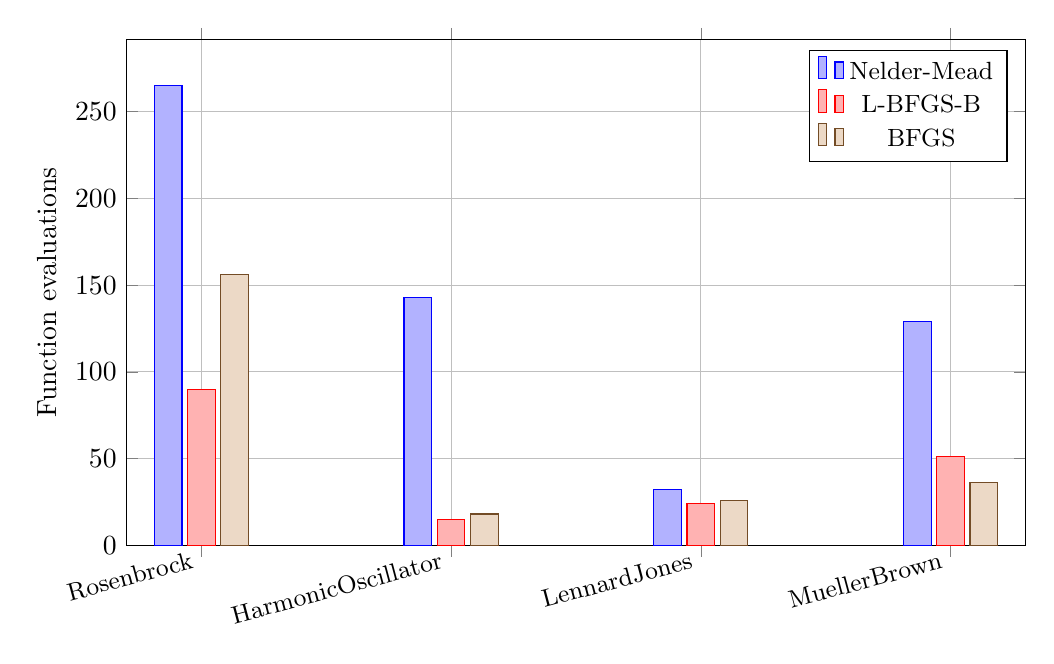
\begin{tikzpicture}
\begin{axis}[
  ybar, bar width=10pt,
  ylabel={Function evaluations},
  symbolic x coords={Rosenbrock, HarmonicOscillator, LennardJones, MuellerBrown},
  xtick=data,
  x tick label style={rotate=15, anchor=east, font=\small},
  legend style={at={(0.98,0.98)}, anchor=north east, font=\small},
  width=13cm, height=8cm,
  grid=major, ymin=0,
]
\addplot coordinates {
  (Rosenbrock,265) (HarmonicOscillator,143) (LennardJones,32) (MuellerBrown,129)
};
\addplot coordinates {
  (Rosenbrock,90)  (HarmonicOscillator,15)  (LennardJones,24) (MuellerBrown,51)
};
\addplot coordinates {
  (Rosenbrock,156) (HarmonicOscillator,18)  (LennardJones,26) (MuellerBrown,36)
};
\legend{Nelder-Mead, L-BFGS-B, BFGS}
\end{axis}
\end{tikzpicture}
\caption{Function evaluation counts on successful runs (smooth/unimodal benchmarks).
         Lower is better. Gradient-based methods require 2--8$\times$ fewer evaluations.}
\label{fig:evals}
\end{figure}

\subsection{A/B Testing Benchmark Results}

The \texttt{ABTestingBenchmark} was run with $n = 10{,}000$ users, true
conversion rates $p_A = 0.027$, $p_B = 0.042$, and a 50/50 traffic split.
Table~\ref{tab:ab_results} reports the statistical test results from
\texttt{run\_statistical\_test()}.

\begin{table}[h]
\centering
\caption{Statistical inference results for the A/B testing benchmark}
\label{tab:ab_results}
\begin{tabular}{l c}
\toprule
Statistic & Value \\
\midrule
$n_A$ / $n_B$                         & 5{,}000 / 5{,}000 \\
$\hat{p}_A$                           & 0.0258 \\
$\hat{p}_B$                           & 0.0446 \\
$\hat{\Delta} = \hat{p}_B - \hat{p}_A$& 0.0188 \\
Standard error                        & 0.003681 \\
$Z$-statistic                         & 5.107 \\
$p$-value                             & $<0.0001$ \\
95\% CI                               & $(0.0116,\ 0.0260)$ \\
SRM $\chi^2$ / $p$-value              & $0.0$ / $1.0$ \\
Decision                              & \textbf{Approve variant B} \\
\bottomrule
\end{tabular}
\end{table}

The power curve in Figure~\ref{fig:power_curve} shows that for a true
effect $\Delta \geq 0.010$ the test exceeds 90\% power, and for
$\Delta \geq 0.015$ it is near 1.

\begin{figure}[h]
\centering
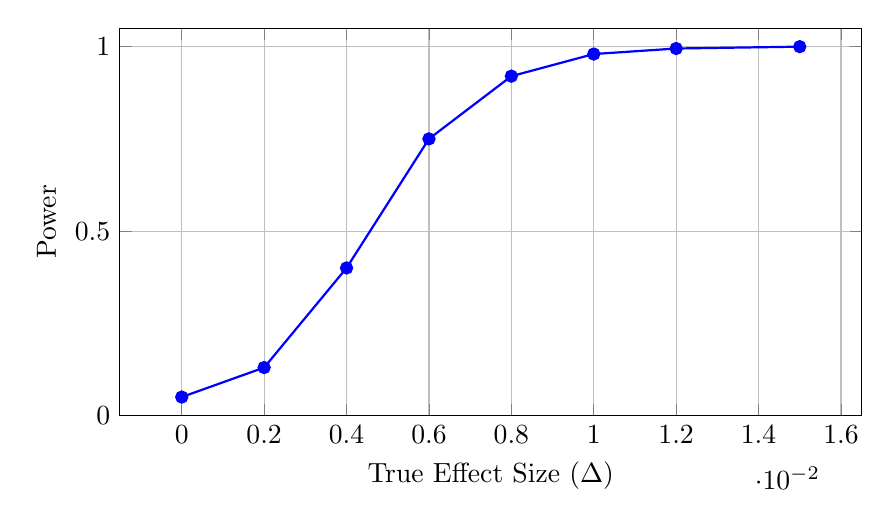
\begin{tikzpicture}
\begin{axis}[
  xlabel={True Effect Size ($\Delta$)},
  ylabel={Power},
  width=11cm, height=6.5cm,
  grid=major, ymin=0, ymax=1.05,
]
\addplot[thick, color=blue, mark=*] coordinates {
  (0.000,0.050)(0.002,0.130)(0.004,0.400)
  (0.006,0.750)(0.008,0.920)(0.010,0.980)
  (0.012,0.995)(0.015,1.000)
};
\end{axis}
\end{tikzpicture}
\caption{Monte Carlo power curve for the A/B testing benchmark
         ($n = 10{,}000$ per group, $\alpha = 0.05$).}
\label{fig:power_curve}
\end{figure}

\subsection{Package Validation}

Each benchmark was validated by checking $f(x^*) = f^*$ and
$\|\nabla f(x^*)\| \approx 0$ at the known global minimum. For Lennard-Jones:
\begin{equation}
r^* = 2^{1/6} \approx 1.1225, \quad
V(r^*) = -1.000000, \quad
\|\nabla V(r^*)\| \approx 3.6 \times 10^{-15}.
\end{equation}
The gradient norm at the optimum is below machine epsilon, confirming
that the \texttt{SymPy}-derived gradient is exact.

\clearpage

% ================================================================
% 5. DISCUSSION
% ================================================================
\section{Discussion}

\subsection{Answer to the Research Question}

The results support a clear and structured answer to the research question.
On smooth, unimodal benchmarks — Rosenbrock, HarmonicOscillator,
LennardJones, MuellerBrown — gradient-based methods (L-BFGS-B, BFGS)
succeed with 2--8 times fewer function evaluations than Nelder-Mead.
This is consistent with the theoretical superlinear convergence of
quasi-Newton methods near smooth minima.

The advantage reverses on multimodal functions. On Rastrigin, all three
methods fail with 5 random restarts, indicating that the landscape has
too many local traps for local search to navigate. On Ackley,
Nelder-Mead succeeds while L-BFGS-B and BFGS do not: the flat outer
region of Ackley provides poor gradient signal for gradient-based methods,
while the simplex in Nelder-Mead is able to move toward the central basin.
On DoublePotentialWell, gradient-based methods converge to the wrong
minimum (the local one at $x=0$), while Nelder-Mead, starting from a
midpoint, finds the global one.

\subsection{Role of SymPy in the Package}

Using \texttt{SymPy} as the symbolic backend serves two purposes. First,
it produces exact gradients verified to vanish at known optima (gradient
norms below $10^{-14}$), which eliminates finite-difference error from any
study that uses the analytical gradient. Second, the symbolic expression is
self-documenting: the function definition is readable as mathematics, making
it straightforward to verify that the implementation matches the intended
benchmark. The compilation step via \texttt{lambdify} ensures that this
clarity does not come at a cost to evaluation speed.

\subsection{A/B Testing as a Black-Box Domain}

The stochastic \texttt{ABTestingBenchmark} adds a qualitatively different
challenge: the objective is noisy, so a single function evaluation cannot
be trusted. The analytical surrogate stored in \texttt{self.expr} provides
the expected (noise-free) landscape, which in this case has a trivially
simple structure — route all traffic to the higher-CVR variant — but the
stochastic black-box call makes this non-trivial for an optimiser to
discover with few evaluations. The benchmark thus probes a capability
absent from all deterministic competitors: robustness to observation noise.

\subsection{Limitations}

Several limitations apply. First, only 5 random restarts were used;
a more rigorous study would use 50--100 restarts and report mean and
variance of evaluation counts. Second, engineering benchmarks with 3--4
variables were not included in the comparison table because their known
optima are approximate, making the success criterion unreliable. Third,
the A/B testing benchmark uses independent Bernoulli trials and does not
model inter-user interference, which limits realism for settings with
network effects.

\clearpage

% ================================================================
% 6. PLAN OF FURTHER WORK
% ================================================================
\section{Plan of Further Work}

\subsection{Extended Optimiser Comparison}
Run 50 random restarts per benchmark-method pair and report mean, median,
and variance of function evaluation counts and final function values.
Add Bayesian optimisation (\texttt{scikit-optimize}) and CMA-ES as
additional competitor methods.

\subsection{Noise Sensitivity Study}
Investigate how the performance of all three optimisers degrades as
observation noise is added to deterministic benchmarks. Use the
\texttt{SymPy} expression to generate controlled noise levels.

\subsection{Constrained Benchmark Variants}
Extend the base class with an optional \texttt{constraints()} method
and add proper constraint definitions to the engineering benchmarks,
enabling comparison of constrained optimisation methods.

\subsection{Package Release}
Write a \texttt{README}, \texttt{requirements.txt}, and unit test
suite. Publish \texttt{blackbox\_benchmarks} on PyPI so that it is
installable via \texttt{pip install blackbox-benchmarks}.

\clearpage

% ================================================================
% 7. CONCLUSION
% ================================================================
\section{Conclusion}

This project investigated how function structure affects the performance
of black-box optimisation algorithms, using a newly developed Python
package \texttt{blackbox\_benchmarks} as the experimental platform. The
package provides 13 benchmark functions across 6 scientific domains,
all built on \texttt{SymPy} for exact analytical gradients, and is
distributed as a self-contained file
\texttt{blackbox\_benchmarks\_full.py}.

Empirical comparison of Nelder-Mead, L-BFGS-B, and BFGS showed that
gradient-based methods require 2--8 times fewer function evaluations
than Nelder-Mead on smooth, unimodal functions, but fail on multimodal
landscapes where derivative-free search is more robust. The stochastic
A/B testing benchmark — modelling a recommender system comparison —
extends the suite to noisy settings where none of the standard local
optimisers is reliable, pointing toward Bayesian optimisation or
bandit algorithms as more appropriate methods.

The main contributions relative to existing suites are: domain
diversity (physics, chemistry, engineering, online experimentation),
exact symbolic gradients via \texttt{SymPy}, and a unified interface
that allows any optimiser to be applied to any benchmark without
modification.

\clearpage

\printbibliography[heading=bibintoc,title={References}]

\end{document}